\documentclass[12pt]{article}
\usepackage{fullpage}
\usepackage{graphicx}
\usepackage{amsfonts}
\usepackage{color}
\usepackage{soul}
\pagestyle{plain}
\setlength{\oddsidemargin}{0.5in}
\setlength{\evensidemargin}{0.5in}
\setlength{\textwidth}{6.0in}
\renewcommand{\baselinestretch}{1.2}
\newcommand{\Dsl}{{\not\!\! D}}
\newcommand{\psl}{{\not\! p}}
\usepackage{gensymb}
\usepackage{tikzsymbols}
\usepackage[utf8]{inputenc}
\usepackage{array}
\usepackage{makecell}
\usepackage{hyperref}

\renewcommand\theadalign{bc}
\renewcommand\theadfont{\bfseries}
\renewcommand\theadgape{\Gape[4pt]}
\renewcommand\cellgape{\Gape[4pt]}

%Above are the packages that are needed for most of the reports that you will write
%%%%%%%%%%%%%%%%%%%%%%%%%%%%%%%%%%%%%%%%%%%



\title{Kinematics One}
\author{Kody Rogers}
\date{\today}
\begin{document}

\maketitle
\thispagestyle{empty}

%Above is title stuff
%%%%%%%%%%%%%%%%%%%%%%%%%%%%%%%%%%%%%%%%%%%%%

\section{Definitions}
\subsection{Vectors}
Let's start with an example.

Someone  is driving North 30 $\degree$ East and that coordinate system is described in the figure below.

\begin{figure}[h]
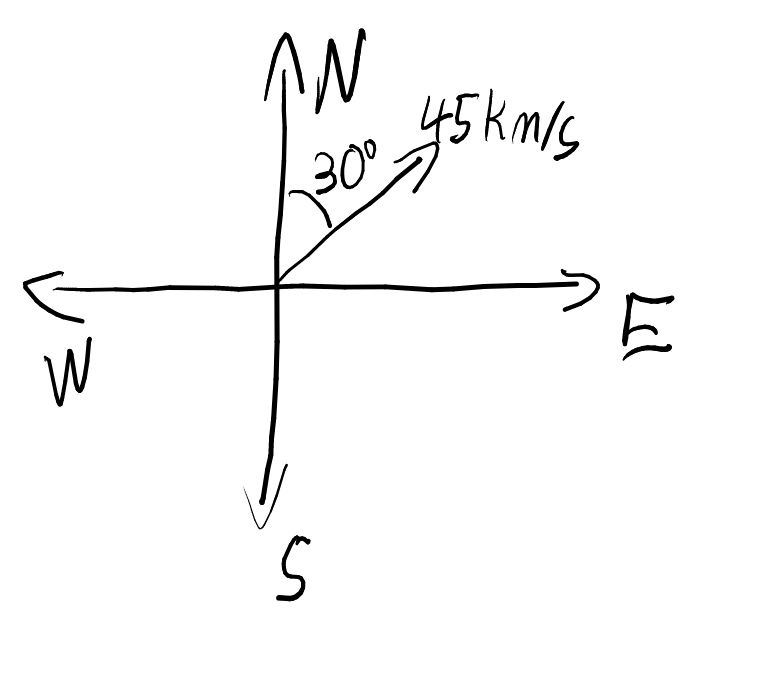
\includegraphics[scale=0.25]{firstVelocityDiagram.png}
\end{figure}

The speed at which the driver is going is $45 \frac{km}{s}$. In this case the speed is what is called the magnitude. When we give a direction, as in the first statement, it is made into a vector.

In this case the vector can be split into a North part and an East part using trigonometry. I will start doing that below by writing done the triangle in question.

\begin{figure}[h]
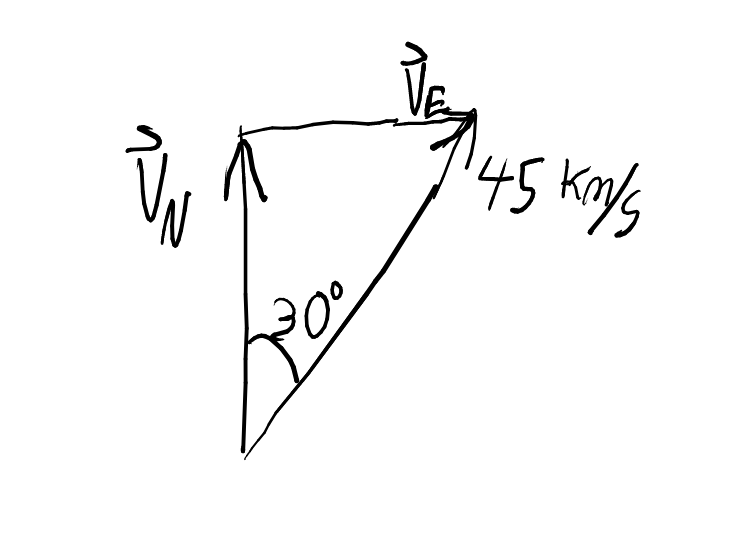
\includegraphics[scale=0.25]{velocityTriangle.png}
\end{figure}

Now you can find the East and the North parts by using what was learned from the trigonometry worksheet.

\parbox[][12cm][t]{8cm}{}

\subsection{Position}
A position is a location. For example 2m N and 1 m E of the main doors on the North end of the Northern Lights Palace in Melfort, Saskatchewan, Canada is a position which someone could be standing.

\begin{figure}[h]
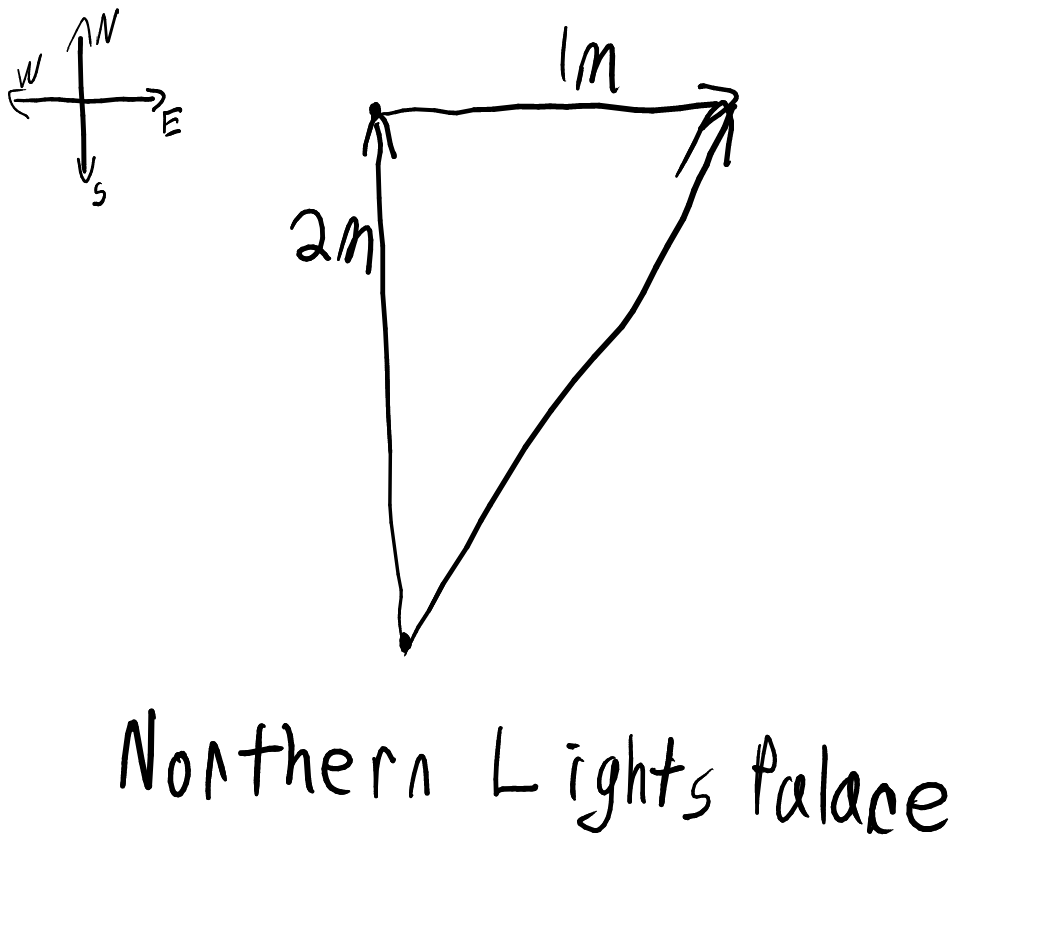
\includegraphics[scale=0.20]{NLPposition.png}
\end{figure}

For practice write down two other possible positions. Remember always mention a reference point (in physics lingo this is called the origin).

\parbox[][12cm][t]{8cm}{}

P.S. It is always a good idea to define a coordinate system as well. A coordinate system is way to define how far things are from the origin and in what direction. In my example I used the North, East, South, West coordinate system because it is well defined and most people are familiar with it. There are more general coordinate systems such as the Cartesian coordinate system, and I encourage the reader to seek out more information about them.

\subsection{Velocity}
Velocity is the rate of change in position. So when you tell someone that you are driving $100 \frac{km}{hour}$ towards you they are giving you a velocity. The $100 \frac{km}{hour}$ is the magnitude of velocity, commonly refered to as speed, and 'towards you' is the direction. The direction combined with the magnitude makes the quoted value a vector.

If we continue with the example involving the Northern Lights Palace we can dig deeper. Let's say you want to go to the library which is just across the street and roughly North in direction, so you start walking there at a pace of $1 \frac{m}{s}$ North. In this case North is the direction and $1 \frac{m}{s}$ is the magnitude. If the library is exactly 20m North from the Northern lights palace how low will it take you to get there.

\parbox[][12cm][t]{8cm}{}

\subsection{Acceleration}
Acceleration is the rate of change of the velocity. If you wanted to get to the library faster you would try and speed up, that is accelerate. Say decided to add an extra $1 \frac{m}{s}$ to your velocity in the Northern direction for every second that goes by. Then it would be said you have an acceleration of $1 \frac{m}{s^2}$ North.

The position is now given as:

$d = v_0t + \frac{1}{2}at^2$

Where, t = the time in seconds, a = the acceleration, and $v_0$ = the original velocity. The reason for the $\frac{1}{2}$ is difficult to explain without calculus, so I will leave that explanation for another worksheet.

Now how fast can you get to the library? (Hint you will need the quadratic equation)

\parbox[][12cm][t]{8cm}{}

\section{Free Fall}
In a vacuum everything accelerates towards the Earth at the same acceleration. That is what is refered to as "free-fall", as in when something is falling towards the Earth with no other forces affecting the object. For example take a feather and a bolder, neglecting air resistance, they will hit the ground at the same time if released at the same height. The acceleration which is relevant here is $g = 9.80 \frac{m}{s^2}$. The interested reader should refer to some more in depth discussions about why this acceleration is roughly constant near Earh here:

\begin{enumerate}
  \item \href{http://hyperphysics.phy-astr.gsu.edu/hbasees/Class/PhSciLab/freefall.html}{HyperPhysics: Free Fall}
  \item \href{https://www.khanacademy.org/science/ap-physics-1/ap-one-dimensional-motion/falling-objects-ap-physics/a/freefall-ap1}{Khan Academy: Free Fall}
\end{enumerate}

Now lets do an example! Say an apple is released from a height of 10 m and a couch is released from the same height at the same time. How long, neglecting air resistance, does it take them to hit the ground? Why do you not need the masses?

\parbox[][12cm][t]{8cm}{}

\section{A More Accurate Canon}
A canon is aimed to fire a canon ball at an angle of 30 degrees with respect to the ground as shown in the diagram.

\begin{figure}[h]
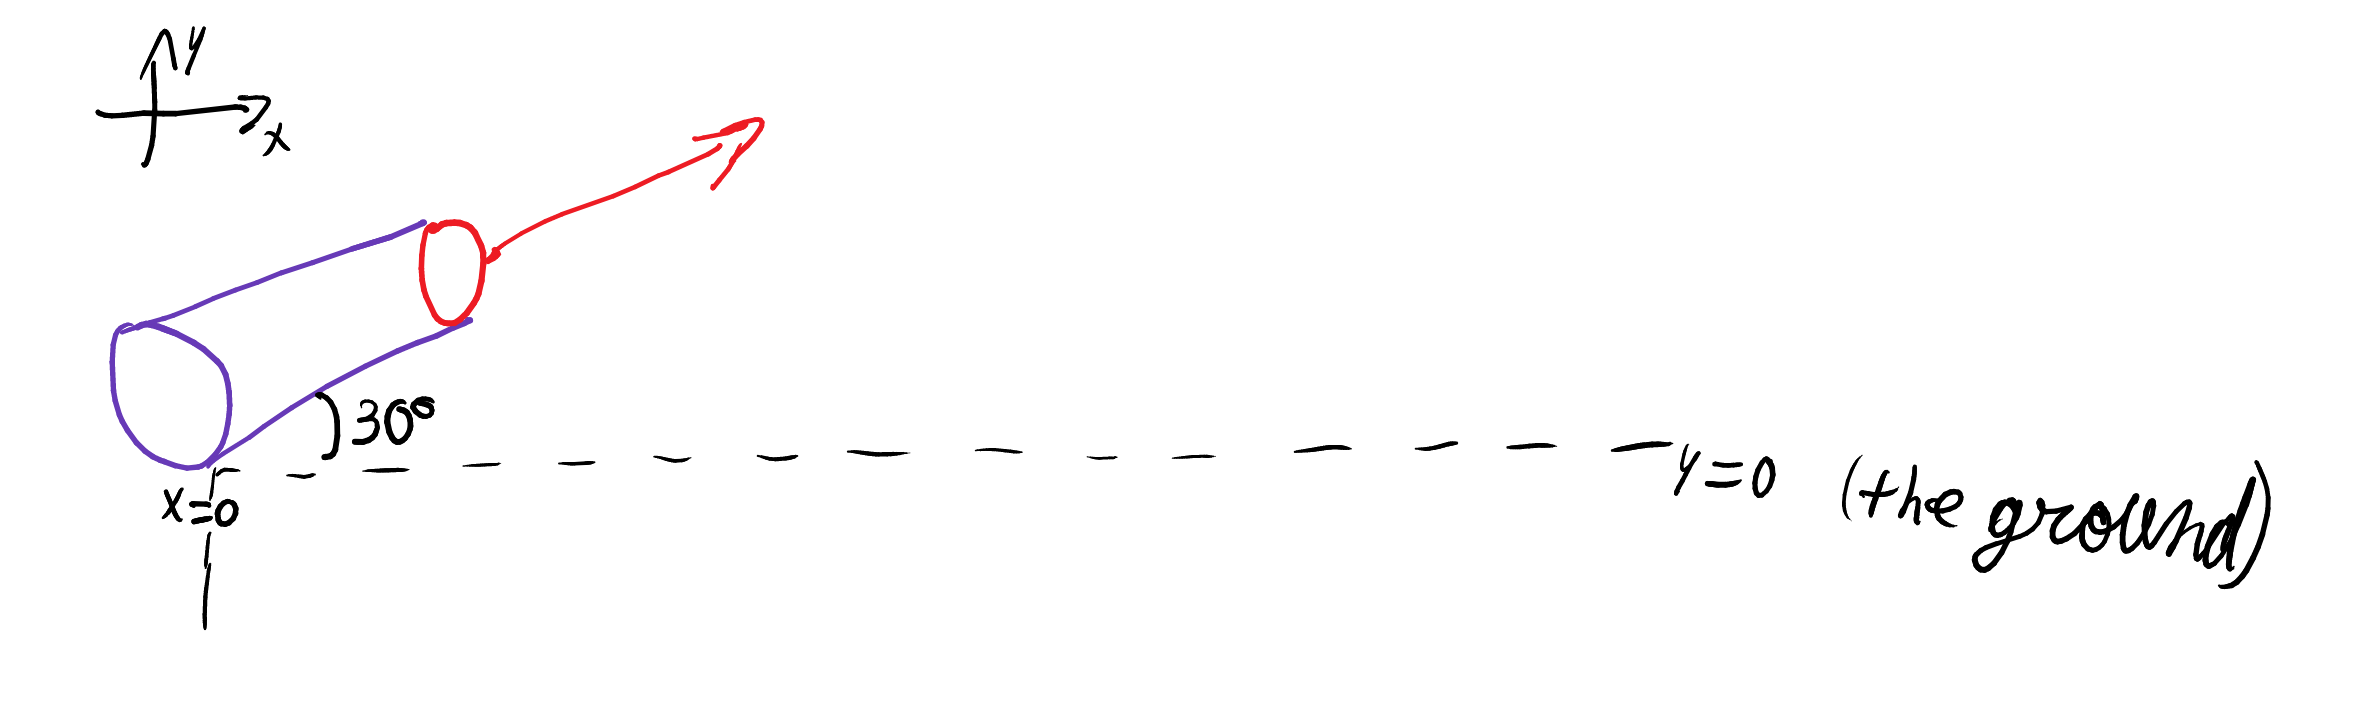
\includegraphics[scale=0.20]{TheCanons.png}
\end{figure}

First what is the velocity in the x-direction, and the y-direction? What about the respective accelerations?

\parbox[][12cm][t]{8cm}{}

How high does the canon ball rise to before gravity reverses its acceleration? How long will it take the for the canon ball to fall to the ground?

\newpage

How far will the canon ball travel in the x-direction?

\parbox[][6cm][t]{8cm}{}

What would happen if the canon was elevated (like on a castle wall or something)? What would happen if the angle was steeper? More gradual? Where does the energy from the canon ball go (Hint: you many need to research conservation of energy)?

\parbox[][12cm][t]{8cm}{}

\section{Who will win?}
Two brothers are out snowmobiling. They have one new snowmobile and one old snowmobile. Both brothers are amazed at the acceleration of the new snowmobile, and want to test it out by racing the two snowmobiles. A fair race would not make sense since the new snowmobile would win very easily, so they set up a rigged one.

The brothers are out in a field that stretches 1 km in total so there is lots of runway. They decide to divide the race into two parts. The old snowmobile gets 500m to get up to its top speed and the new snowmobile waits until the old one passes it and then it starts accelerating. The time that the new snowmobile we will call $t=0$. The sitution is described below in the diagram.

\begin{figure}[h]
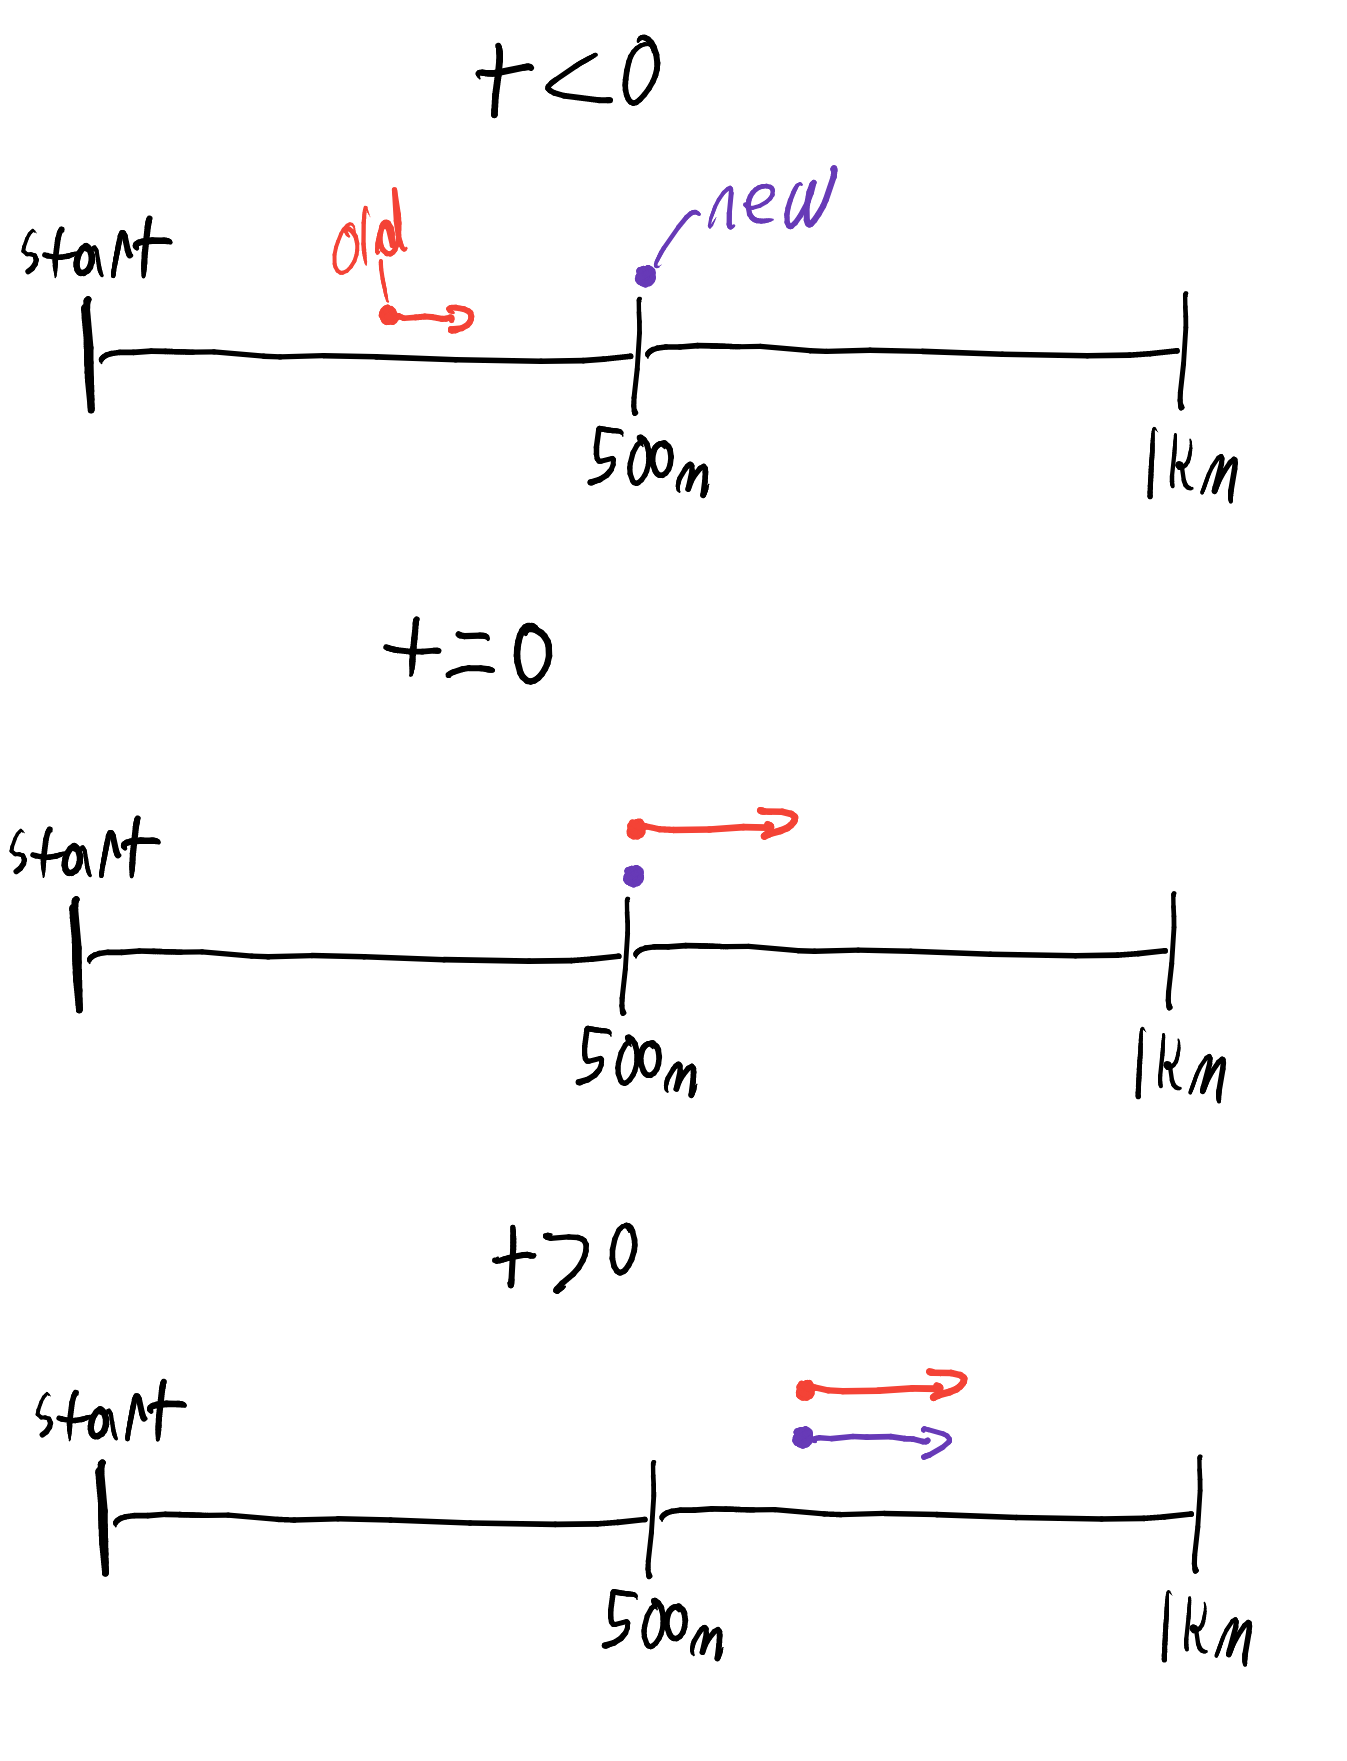
\includegraphics[scale=0.15]{snowmobileRally.png}
\end{figure}

For $t > 0$ the old snowmobile does not accelerate and moves along at the velocity of $v_{old} = 30 \frac{km}{hour} xhat$. The xhat means it is going in the x direction as defined in the diagram. The new snomobile is accelerating in the same direction as the old snowmobile at a rate of $a_{new} = 6\frac{km}{s}$

Who wins the race? What speed does the new snowmobile get to? Is it realistic that the new snowmobile never stops accelerating during the race? How accurate is my diagram? (room for work on the next page)

\parbox[][12cm][t]{8cm}{}

\section{Who hit further?}
Two batters hit a baseball in the same baseball field. To hit a home run you have to hit the baseball 100m in positive x direction (defined in the next diagram).

The first baseball player hits the ball at a 30 degree angle with respect to the ground at a speed of 70$\frac{km}{hr}$. Below is a diagram showing the angle and speed of the first ball.

- add the diagram

A good first step would be to convert the speed from $\frac{km}{hr}$ to $\frac{m}{s}$ as follows:

$v_1 = (70 \frac{km}{hr})(\frac{1000m}{1km})(\frac{1hr}{3600s}) = 19.4 \frac{m}{s}$

In the above equation we used the fact that $1km = 1000m$ and that $1hr = 3600s$ to convert to $\frac{m}{s}$

The other batter hits the ball at a 30 degree angle with respect to the ground and with a speed of $80 \frac{km}{hr}$.


Which ball goes further? Do either of them hit a home run?

Hint: Refer to the canon ball problem, draw a picture for the second batter and for the home run question, and make sure all speeds are in $\frac{m}{s}$

%Above is the Discussion
%%%%%%%%%%%%%%%%%%%%%%%%%%%%%%%%%%%%%%%%%%%%%%%%%%%%%%%
\end{document}
